\documentclass{beamer}
\usepackage[T1]{fontenc}
\usepackage[utf8]{inputenc}

\usetheme{Madrid}
\usecolortheme{default}
\usepackage{amsmath,amssymb,amsfonts,amsthm}
\usepackage{mathtools}
\usepackage{txfonts}
\usepackage{tkz-euclide}
\usepackage{listings}
\usepackage{adjustbox}
\usepackage{array}
\UseRawInputEncoding
\usepackage{multicol}
\usepackage{gensymb}
\usepackage{tabularx}
\usepackage{gvv}
\usepackage{lmodern}
\usepackage{circuitikz}
\usepackage{tikz}
\lstset{literate={·}{{$\cdot$}}1 {λ}{{$\lambda$}}1 {→}{{$\to$}}1}
\usepackage{graphicx}

\setbeamertemplate{page number in head/foot}[totalframenumber]

\usepackage{tcolorbox}
\tcbuselibrary{minted,breakable,xparse,skins}


\definecolor{bg}{gray}{0.95}
\DeclareTCBListing{mintedbox}{O{}m!O{}}{%
  breakable=true,
  listing engine=minted,
  listing only,
  minted language=#2,
  minted style=default,
  minted options={%
    linenos,
    gobble=0,
    breaklines=true,
    breakafter=,,
    fontsize=\small,
    numbersep=8pt,
    #1},
  boxsep=0pt,
  left skip=0pt,
  right skip=0pt,
  left=25pt,
  right=0pt,
  top=3pt,
  bottom=3pt,
  arc=5pt,
  leftrule=0pt,
  rightrule=0pt,
  bottomrule=2pt,
  toprule=2pt,
  colback=bg,
  colframe=orange!70,
  enhanced,
  overlay={%
    \begin{tcbclipinterior}
    \fill[orange!20!white] (frame.south west) rectangle ([xshift=20pt]frame.north west);
    \end{tcbclipinterior}},
  #3,
}
\lstset{
    language=C,
    basicstyle=\ttfamily\small,
    keywordstyle=\color{blue},
    stringstyle=\color{orange},
    commentstyle=\color{green!60!black},
    numbers=left,
    numberstyle=\tiny\color{gray},
    breaklines=true,
    showstringspaces=false,
}
\title{8.4.13}
\subtitle{Ellipse and hyperbola}
\author{EE25BTECH11010 - Arsh Dhoke}
\date{}
\begin{document}

\frame{\titlepage}

\begin{frame}{Question}
Let a hyperbola passes through the focus of the ellipse 
\[
\frac{x^2}{25} + \frac{y^2}{16} = 1.
\]
The transverse and conjugate axes of this hyperbola coincide with the major and minor axes of the given ellipse, also the product of eccentricities of given ellipse and hyperbola is 1, then
\begin{multicols}{2}
\begin{enumerate}
    \item the equation of hyperbola is 
    $\frac{x^2}{9} - \frac{y^2}{16} = 1$
    \item the equation of hyperbola is 
    $\frac{x^2}{9} - \frac{y^2}{25} = 1$
    \item focus of hyperbola is $(5, 0)$
    \item vertex of hyperbola is $(5\sqrt{3}, 0)$
\end{enumerate}
\end{multicols}
\end{frame}

\begin{frame}{Solution}
The general equation of the conic can be written as:
\begin{align}
\vec{x^T}\vec{V}\vec{x} + 2\vec{u^T}\vec{x} + f = 0
\end{align}

\begin{align}
\vec{V}_E=\myvec{\frac{1}{25}&0\\0&\frac{1}{16}}, \quad \vec{u}=\vec{0}, \quad f=-1
\end{align}

\begin{align}
\lambda_1=\frac{1}{25}, \quad \lambda_2=\frac{1}{16}
\end{align}

\begin{align}
e_E^2 = 1 - \frac{\lambda_1}{\lambda_2}, \quad 
e_E = \frac{3}{5}
\end{align}

\begin{align}
e_H \cdot e_E = 1 \Rightarrow e_H = \frac{5}{3}, \quad e_H^2 = \frac{25}{9}
\end{align}
\end{frame}

\begin{frame}{Calculating parameters for Hyperbola}
\begin{align}
\vec{V}_H = \myvec{\lambda_1' & 0 \\ 0 & \lambda_2'}, \quad f = -1
\end{align}

Hyperbola passes through  (3,0), thus
\begin{align}
9\lambda_1' - 1 = 0 \Rightarrow \lambda_1' = \frac{1}{9}
\end{align}

\begin{align}
e_H^2 = 1 - \frac{\lambda_1'}{\lambda_2'} \Rightarrow \lambda_2' = \frac{\lambda_1'}{1 - e_H^2}
\end{align}

\begin{align}
\lambda_2' = \frac{\frac{1}{9}}{1 - \frac{25}{9}} = \frac{\frac{1}{9}}{-\frac{16}{9}} = -\frac{1}{16}
\end{align}

\begin{align}
\vec{V}_H = \myvec{\frac{1}{9} & 0 \\ 0 & -\frac{1}{16}}
\end{align}
\end{frame}

\begin{frame}{Answer}
\begin{align}
\frac{x^2}{9} - \frac{y^2}{16} = 1
\end{align}

\begin{align}
b'^2 = 16, \quad 
c = \sqrt{\frac{\abs{\lambda_1' - \lambda_2'}}{\abs{\det{\vec{V}}}}}
\end{align}

\begin{align}
c = 5
\end{align}

\begin{align}
\text{Foci: } \myvec{\pm5 \\ 0}, \quad \text{Vertices: } \myvec{\pm3 \\ 0}
\end{align}

\begin{align}
\boxed{\text{Correct options: (1) and (3)}}
\end{align}
\end{frame}

\begin{frame}{Graph}
\begin{figure}
\centering
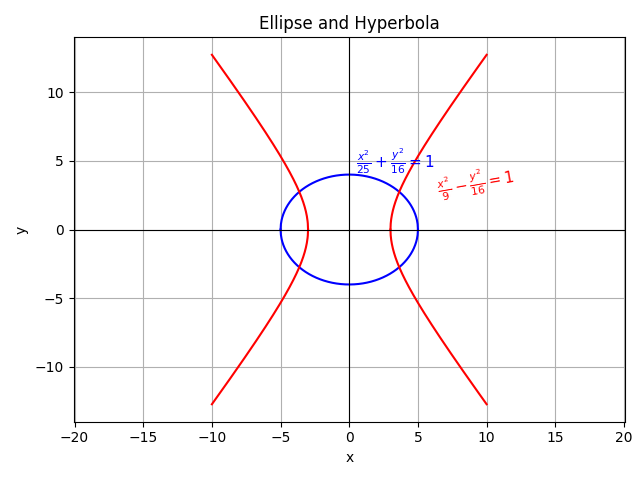
\includegraphics[height=0.4\textheight, keepaspectratio]{figs/ell.png}
\caption{Graph}
\end{figure}
\end{frame}

\begin{frame}[fragile]
    \frametitle{C Code}
\begin{lstlisting}
#include <stdio.h>
#include <math.h>

void solve_conic() {
    double a_ellipse = 5.0, b_ellipse = 4.0;
    double e_E = sqrt(1 - (b_ellipse * b_ellipse) / (a_ellipse * a_ellipse));
    double e_H = 1.0 / e_E;
    double eH2 = e_H * e_H;

    double x = 3.0;
    double lambda1_H = 1.0 / (x * x);
    double lambda2_H = lambda1_H / (1 - eH2);

    double a_H = sqrt(1.0 / lambda1_H);
    double b_H = sqrt(-1.0 / lambda2_H);
    double c_H = sqrt(a_H * a_H + b_H * b_H);

}
\end{lstlisting}
\end{frame}

\begin{frame}[fragile]
    \frametitle{Python Code}
\begin{lstlisting}
import numpy as np
import matplotlib.pyplot as plt

# Ellipse parameters
a_ellipse = 5
b_ellipse = 4

# Hyperbola parameters
a_hyperbola = 3
b_hyperbola = 4

# Ellipse: x ∈ [-a, a]
x_ellipse = np.linspace(-a_ellipse, a_ellipse, 400)
y_ellipse = b_ellipse * np.sqrt(1 - (x_ellipse / a_ellipse)**2)

# Hyperbola: valid only for |x| ≥ a
x_right = np.linspace(a_hyperbola, 10, 400)
x_left = np.linspace(-10, -a_hyperbola, 400)

y_right = b_hyperbola * np.sqrt((x_right / a_hyperbola)**2 - 1)
y_left  = b_hyperbola * np.sqrt((x_left  / a_hyperbola)**2 - 1)
\end{lstlisting}
\end{frame}

\begin{frame}[fragile]
    \frametitle{Python Code}
\begin{lstlisting}
# Plot ellipse
plt.plot(x_ellipse,  y_ellipse, 'b', label='Ellipse')
plt.plot(x_ellipse, -y_ellipse, 'b')

# Plot hyperbola (both branches)
plt.plot(x_right,  y_right, 'r', label='Hyperbola')
plt.plot(x_right, -y_right, 'r')
plt.plot(x_left,   y_left,  'r')
plt.plot(x_left,  -y_left,  'r')

# Axes
plt.axhline(0, color='k', linewidth=0.8)
plt.axvline(0, color='k', linewidth=0.8)

# Labels and formatting
plt.xlabel('x')
plt.ylabel('y')
plt.title('Ellipse and Hyperbola')
\end{lstlisting}
\end{frame}

\begin{frame}[fragile]
    \frametitle{Python Code}
\begin{lstlisting}
plt.axis('equal')
plt.grid(True)
plt.tight_layout()

# Annotate equations beside curves
plt.text(6.2, 2.5, r'$\frac{x^2}{9} - \frac{y^2}{16} = 1$', color='r', fontsize=11, rotation=10)
plt.text(0.5, 4.5, r'$\frac{x^2}{25} + \frac{y^2}{16} = 1$', color='b', fontsize=11)
plt.savefig("/home/arsh-dhoke/ee1030-2025/ee25btech11010/matgeo/8.4.13/figs/ell.png")
plt.show()

\end{lstlisting}
\end{frame}

\begin{frame}[fragile]
    \frametitle{Python+ C Code}
\begin{lstlisting}
import ctypes
import numpy as np
import matplotlib.pyplot as plt

# Load the shared library
lib = ctypes.CDLL('./code.so')

# Define the function signature
lib.solve_conic.restype = None

# Call the function
lib.solve_conic()

# Ellipse parameters
a_e, b_e = 5, 4
theta = np.linspace(0, 2*np.pi, 400)
x_ellipse = a_e * np.cos(theta)
y_ellipse = b_e * np.sin(theta)
\end{lstlisting}
\end{frame}

\begin{frame}[fragile]
    \frametitle{Python+ C Code}
\begin{lstlisting}
# Hyperbola parameters
a_h, b_h = 3, 4
x_vals = np.linspace(-10, 10, 400)
y_hyperbola_pos = b_h * np.sqrt((x_vals**2 / a_h**2) - 1)
y_hyperbola_neg = -y_hyperbola_pos

# Plot
plt.figure(figsize=(6,6))
plt.plot(x_ellipse, y_ellipse, 'b', label=r'$\frac{x^2}{25} + \frac{y^2}{16} = 1$')
plt.plot(x_vals, y_hyperbola_pos, 'r', label=r'$\frac{x^2}{9} - \frac{y^2}{16} = 1$')
plt.plot(x_vals, y_hyperbola_neg, 'r')

# Annotate
plt.text(6, 0.5, r'$\frac{x^2}{9} - \frac{y^2}{16} = 1$', color='r')
\end{lstlisting}
\end{frame}

\begin{frame}[fragile]
    \frametitle{Python+ C Code}
\begin{lstlisting}
plt.text(2, 3.5, r'$\frac{x^2}{25} + \frac{y^2}{16} = 1$', color='b')

# Styling
plt.axhline(0, color='k', lw=0.8)
plt.axvline(0, color='k', lw=0.8)
plt.axis('equal')
plt.xlabel('x')
plt.ylabel('y')
plt.title('Ellipse and Hyperbola')
plt.grid(True)
plt.savefig("/home/arsh-dhoke/ee1030-2025/ee25btech11010/matgeo/8.4.13/figs/ell.png")
plt.show()

\end{lstlisting}
\end{frame}
\end{document}
